\chapter{Introducción}
\graphicspath{{figs/cap1/}}
\label{cap1}



En el estudio de la Mecánica de los Fluidos, son de importancia los problemas de transferencia de calor de flujos multi-fásicos con cambios de fase. 
Los problemas presentan la particularidad que se han realizado ensayos experimentales que estudian la fenomenología del mismo. \textbf{que queres decir con esto?}s

Para los tipos de problemas mencionados no se posee actualmente algún método numérico que concuerde con los ensayos realizados y sea producido en un tiempo aceptable. \textbf{Es una idea vaga}

Un ejemplo de aplicacion industrial del tipo de problema mencionado rescide en el estudio de un reactor nuclear. La transferencia de calor producida en las barras de elementos combustibles del núcleo provoca ebullición nucleada a partir de una dada potencia. Se conoce bien cómo es la fenomenología en función de la potencia entregada, por haberse realizado numerosos ensayos y caracterizado distintos parámetros. 

Actualmente el dilema para reproducir numéricamente los tipos de problemas mencionados es que debido a la escala del fluido (\textit{mesoscópica}) con las técnicas convencionales de resolución de Mecánica de Fluidos Computacional(\textit{Computational Fluid Dynamicso} CFD) no se obtienen resultados en un tiempo razonable y que también tenga en cuenta todos las interacciones físicas que ocurren.

Uno de los métodos numéricos que se están desarrollando para que el costo computacional sea cada vez menor es el método de lattice-Boltzmann. Dicho método tiene la ventaja de ser paralelizable y así disminuir los tiempos de cálculo. \textbf{No es la unica ventaja, porque los metodos tradicionales, como diferencias finitas o volumenes finitos, implican resolver sistemas de ecuaciones lineales. Esto tambi’en es paralelizable. Hay otras ventajas, como poder obtener la solucion de una ecuacion lineal a traves de una edo lineal, o que no es necesario resolver sistemas de ecuaciones (Ax=b), que cuesta mucho computacionalmente. Ver esto en la introduccion de los libros}

\section{Descripción de las escalas de los fluidos}

Los fluidos como el aire y el agua son conocidos en nuestra vida diaria. Físicamente los fluidos están compuestos de un gran conjunto de átomos o moléculas que chocan unas con otras moviéndose  aleatoriamente. Usualmente las interacciones de las moléculas de un fluido son más débiles que las de un sólido, por ello mediante la aplicación de un pequeño esfuerzo al fluido, éste puede ser deformado de manera continua.


Usualmente la dinámica microscópica de las moléculas del fluido son muy complicadas y demuestran una fuerte inhomogeneidad y fluctuaciones.
Por otro lado la dinámica macroscópica del fluido, el cual es el resultado medio del movimiento de las moléculas en un medio homogéneo y continuo.
Mediante modelos matemáticos puede explicarse la dinámica de los fluidos , según el fluido observado y su fuerte dependencia del tamaño de su escala.

La mecánica de los fluidos se puede describir en tres niveles: macroscópica, mesoscópica y microscópica.
Generalmente el movimiento de un fluido puede ser descripto por tres tipos de modelos matemáticos acuerdo a lo que se observan en las distintas escalas, por ejemplo microscópico en modelos de escala molecular, teorías cinéticas en la escala mesoscópica y modelos continuos para escalas macroscópicas.


Los modelos matemáticos de los flujos de fluidos son :

\begin{itemize}
	\item ecuación de Newton para una cantidad elevada de moléculas (escala microscópica)
	\item ecuación de Boltzman para la función de distribución simple (escala mesoscópica)
	\item ecuación de Navier-Stokes para macro-variaciones de flujos (escala macroscópica). \textbf{en todo caso seria alguna aproximacion de continuo. NS es para un tipo de flujo}
\end{itemize}

que resultan extremadamente difíciles de resolver analíticamente de no ser imposibles.

 La precisión de los modelos numéricos sin embargo han provisto de manera satisfactoria soluciones aproximadas de dichas ecuaciones.
Particularmente con la rapidez del desarrollo del software y hardware computacional y la tecnología, las simulaciones numéricas han comenzado a ser una importante metodología para la dinámica de fluidos.

El método más exitoso y popular de simulación de fluidos es la técnica Mecánica de Fluidos Computacional (\textit{Computational Fluid Dynamics} o CFD) , el cual está diseñado para resolver ecuaciones hidrodinámicas basadas en supociones de continuidad.\textbf{No es una tecnica, es una rama de aplicacion/investigacion. Si haces simulaciones de dinamica molecular y de ahi sacas comportamiento de flujo en la escala macro, tambien haces CFD. Tecnicas son diferencias finitas, volumenes finitos, elementos finitos, LB, etc.}
En CFD el dominio del flujo está compuesto en en conjunto de de sub-dominios con una malla computacional, \textbf{hay tecnicas meshless} las ecuaciones matemáticas son discretizadas usando algunos esquemas de discretización numérica como elementos finitos, volúmenes finitos o diferencia finitas; los cuales resultan en un sistema algebraico de sistemas de ecuaciones para las variables discretas del fluido asociadas a la malla computacional. 
Computacionalmente son llevados a cabo para encontrar una solución aproximada resolviendo el problema algebraico de sistemas de ecuaciones usando un algoritmo secuencial o paralelo.
 
La Simulación de Dinámica Molecular (\textit{Molecular Dynamic Simulation} o MDS) es una técnica en la cual el movimiento individual de átomos o moléculas del fluido son registrados para resolver las ecuaciones de Newton.
La principal ventaja de MDS es el aspecto macroscópico del fluido puede ser directamente conectado con el comportamiento molecular, en donde la estructura molecular y las interacciones microscópicas pueden ser descriptas de una manera directa.

El método de lattice Boltzmann ( \textit{lattice Boltzman Method} o LBM) es una aproximación del nivel mesoscópica. LBM estudia la micro-dinámica de partículas ficticias utilizando modelos cinéticos simplificados, lo cual provee un camino alternativo de simular la mecánica de fluidos. La naturaleza de la cinética brinda distintas características de LBM tales que es claro el panorama de los procesos de advección y colisión de partículas de fluidos simuladas. La estructura del algoritmo es simple y de fácil implementación en las condiciones de contorno, además presenta un paralelismo natural. Todos éstos interesantes atributos hacen que LBM sea una potente herramienta numérica para la simulación de sistemas de fluidos envueltos en problemas físicos complejos\cite{guo2013lattice}. 


\section{Descripción general de LBM}

Los modelos de lattice -Boltzmann provienen de la ecuación de Boltzmann, ésta se encuentra discretizada en espacios para resolver los problemas según: espacio físico, espacio de velocidades y espacio temporal. 

La discretización espacial surge de realizar un mallado a la región donde se plantea resolver un dado problema físico, y, cada nodo de la malla tiene asignado un espacio de velocidades. Todos los modelos se encuentran clasificados según el tipo \textit{DdQq} (\textit{d}-dimensiones  \textit{q}-velocidades), siendo \textit{q} la discretización realizada en el espacio de velocidades. La figura \ref{fig:D1Q3_D2Q9} muestra como es el conjunto de velocidades para el modelo D1Q3 y D2Q9.

El espacio de velocidades indica cómo es la propagación de las propiedades que poseen los nodos de la grilla. La velocidad de grilla del nodo i-ésimo se denota $\mathbf{e}_{i}$ y posee \textit{q} componentes. Para el modelo D2Q9 la figura \ref{fig:D1Q3_D2Q9} muestra un esquema de las velocidades de grilla del nodo i - ésimo y la Ec. (\ref{eq:velgrilla}) el valor adoptado.

\begin{figure}[h!]
	\centering
	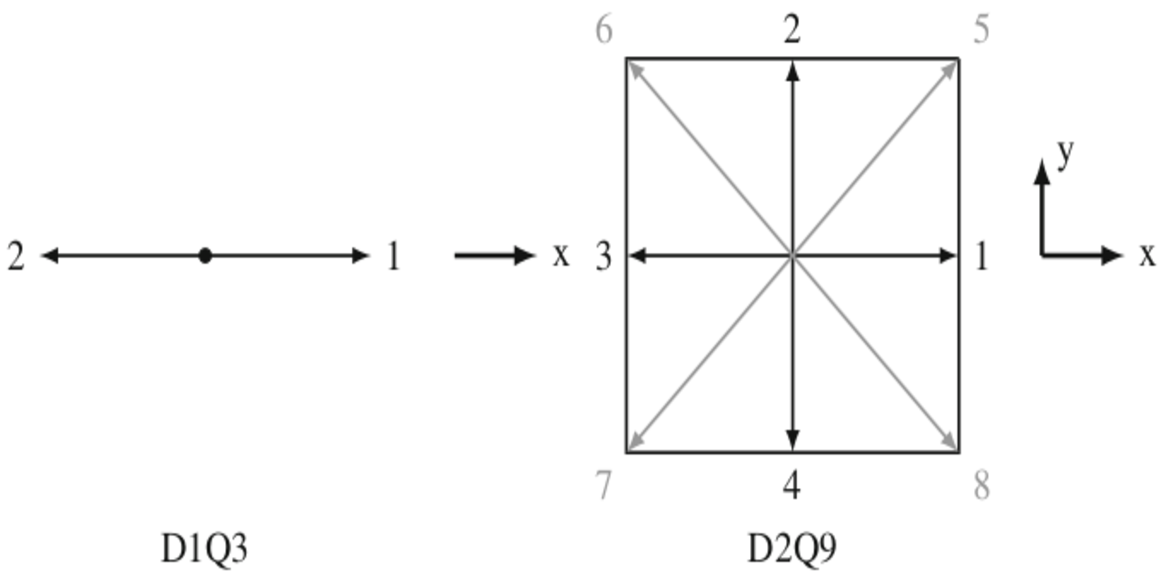
\includegraphics[width=.8\textwidth]{figs/cap1/D1Q3_D2Q9}
	\caption{Conjunto de velocidades de los modelos D1Q3 y D2Q9. \cite{kruger2017lattice}}
	\label{fig:D1Q3_D2Q9}	
\end{figure}


\begin{equation}
{\mathbf{e}}_{i} =  
\left( \begin{array}{c} 
e_{i0} \\ e_{i1}\\ e_{i2}\\ e_{i3}\\ e_{i4}\\ e_{i5}\\
e_{i6}\\ e_{i7}\\ e_{i8}\\
\end{array}
\right) =
\left( \begin{array}{c} 
(0,0,0) \\ (1,0,0) \\ (0,1,0) \\(-1,0,0) \\ (0,-1,0) \\ (1,1,0) \\
(-1,1,0) \\ (-1,-1,0) \\ (1,-1,0)\\ 
\end{array}
\right) 
\label{eq:velgrilla}
\end{equation}




En el presente trabajo se resolverán los problemas descriptos en Cap. \ref{cap4}, los cuáles son de 2 dimensiones y se adoptó el tipo de modelo D2Q9. 



Para los problemas de flujos multifásicos existen cuatro modelos generales de LB , siendo ellos:

\qquad \qquad color gradient, free energy, phase field y pseudopotential.

El modelo que se utilizará en el presente trabajo es el pseudopotencial, el cuál está basado en proponer un potencial de interacción entre las partículas del fluido. El potencial se utiliza para calcular la fuerza de interacción entre las partículas del fluido y está dado según una Ecuación de estado. 

El modelo posee un campo de distribución de probabilidades \textit{f} que tiene asociado \textit{q} componentes, siendo dependiente de la fuerza de interacción. Por medio de \textit{f} se pueden recuperar las variables macroscópicas asociadas del problema a resolver.

A continuación se datallará un ejemplo sencillo de un modelo \textit{D2Q9}. La Figura \ref{fig:grilla_D2Q9} muestra un esquema de las direcciones de las velocidades de grilla del nodo i-ésimo. En la misma figura se esquematiza como  es el proceso de colisión y advección (\textit{streaming}) que se realiza para actualizar los estados de los nodos cuando transcurre un paso de tiempo de la discretización temporal del problema. 


\begin{figure}[h!]
	\centering
	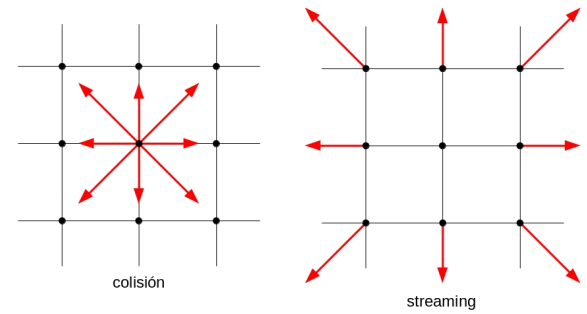
\includegraphics[width=8cm]{grilla_stre_colli_intro.png}
	\caption{Colisión y streaming de un modelo D2Q9 de LBM.}
	\label{fig:grilla_D2Q9}
\end{figure}


\begin{align}
	\mathbf{f}_{\alpha} (\mathbf{x} + \mathbf{e}_{\alpha} \mathbf{\delta}_{t}, t + \mathbf{\delta}_{t})  = \mathbf{f}_{\alpha} (\mathbf{x}, t) - \frac{1}{\tau} (\mathbf{f}_{\alpha} - {\mathbf{f}_{\alpha}}^{eq})
	\label{eq:field_intro} 
\end{align}

El término derecho de la Ec. (\ref{eq:field_intro}) contiene el proceso de \textit{colisión} y el izquierdo al \textit{streaming}; $\alpha$ corresponde al  $\alpha$-ésimo componente de los \textit{q} componentes del modelo, en éste ejemplo $\alpha = 1, 2, ...,9$. $f^{eq}$ es la función de distribución en estado de equilibrio. $\tau$ es un parámetro de relajación del modelo. 

Por medio de la \textit{colisión} y luego del \textit{streaming} se obtienen los parámetros macroscópicos el problema. Para éste caso sencillo se obtiene $\rho$ y $\mathbf{u}$ de las Ec. (\ref{eq: rho.1}) y (\ref{eq: u.1}) respectivamente.

\begin{align}
	\rho = \sum_{\alpha} \mathbf{f}_{\alpha}
	\label{eq: rho.1}
\end{align}

\begin{align}
	\rho \mathbf{u}= \sum_{\alpha} \mathbf{e}_{\alpha} \mathbf{f}_{\alpha}
	\label{eq: u.1}
\end{align}

El método numérico en éste caso tiene los siguiente forma de resolución:
\newline
{\scriptsize

\xymatrix{\>\ar@{->}[r]&\textbf{Colisión}\ar@^{->}[r]&\textbf{Streaming}\ar@{->}[r]&\textbf{C. de Contorno}\ar@{->}[r]&\textbf{Cálculo $\rho$, \textit{F} y \textit{U}\ar@{->}[r]}&\textbf{Actualización$\rho$, \textit{F} y \textit{U}}\ar@{->}[r]&\> \ar@/^{7mm}/[llllll]_{SIGUIENTE \> PASO \> DE \> TIEMPO}}
}
.
\newline 
\newline 

\textbf{Falta condiciones de contorno en el esquema}


\textbf{Qu’e son parametros?}


\textbf{Llegado a este punto no se entiende bien que es LB. Para que se usa, y por que sirve? Es una manera de obtener la solucion de una ecuacion diferencial, pero resolviendo otra que en principio es mas sencilla computacionalmente. Hay que trabajar un poco esta seccion.}

Debido a que cada nodo de la grilla debe realizar la misma operación de colisión de manera independiente del resto, el modelo es altamente paralelizable. Y además las operaciones matemáticas que deben ejecutarse en el operador de colisión son sencillas, no implicando un gran costo computacional.

\textbf{En esta seccion es importante remarcar que despues de la aplicacion del algoritmo LB, el que sea, se obtienen variables macroscopicas cuyo comportamiento queda descripto por las ecuaciones diferenciales de interes. Por eso LB es una manera alternativa de resolver estas ecuaciones. Y hay que destacar tambien que los factores de relajacion se vinculan con propiedades macro, como la viscosidad.}

\newpage
\section{Descripción GPU}

Una Unidad de Procesamiento Gráfico (\textit{Graphics Processing Unit} o GPU) es un  circuito electrónico diseñado para realizar operaciones con punto flotante para renderizar píxeles en una pantalla. Están optimizadas para actuar en paralelo de forma simultánea instrucciones simples.

La GPU trabaja en conjunto con una Unidad Central de Procesamiento (\textit{Central Processing Unit} o CPU), debido a ello no presenta circuitos de control en su arquitectura. Dicho espacio que se encuentra ocupado en las CPU por el circuito de control las GPU lo disponen para incrementar el espacio en su chip de Unidades Aritmético Lógicas (\textit{Arithmetic Logic Unit} o ALU) elevando su poder de cálculo. \textbf{citas}

El esquema de la Figura \ref{fig:cpu_gpu_transis} se muestra cuanlitativamente la cantidade de transistores dedicados a diferentes tareas en la CPU comparado con la GPU.

\begin{figure}[h!]
	\centering
	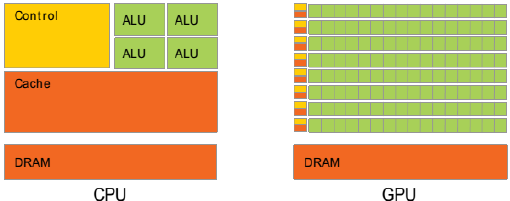
\includegraphics[width=10cm]{cpu_gpu.png}
	\caption{Comparación cualitatica del uso de transistores entre CPU y GPU \cite{rinaldi2011modelos}.}
	\label{fig:cpu_gpu_transis}
\end{figure}

Las GPUs estan acondicionadas para llevar a cabo los cálculos que presentan los métodos numéricos de LB. Los LBM consisten en que a cada uno de los nodos de la grilla discretizada se le realicen operaciones elementales como los de la ecuación \ref{eq:field_intro}. Las GPU se encuentran optimizadas para ejecutar cálculos sobre los píxeles de un monitor, los cuales pueden considerarse como una grilla de nodos. A través de la paralelización la performance de las GPUs es alta, siendo capaces de procesar múltiples vértices y píxeles simultáneamente. Las simulaciones numéricas se producen en un menor tiempo en las GPU que sobre las CPU debido al alto paralelismo alcanzado por la GPU. \cite{rinaldi2011modelos}.


El lenguaje de programación que se utiliza en las placas gráficas es CUDA y fue desarrollado mediante la empresea NVIDIA. Se basa en el lenguaje de programación \textbf{C} con ciertas modificaciones para que los procesos sean en paralelo. Dichos procesos se especifican para que puedan ser lanzados en un número de \textit{blocks} y \textit{threads} de ejecución.






\section{Descripción y alcance del proyecto integrador}

Mediante el método LBM desarrollado por Fogliatto en \cite{fogliatto2018modelado}, \cite{fogliatto2019simulation} y \colorbox{green}{cita de ec energia} se realizó la implementación de un código numérico desarrollado en los lenguajes de programación \textsc{C} y \textsc{CUDA C}; para resolver problemas de transferencia de calor en flujos multifásicos con cambio de fase usando GPU de la forma más robusta posible.

La compilación del código se hizo mediante la herramienta multiplataforma \textsc{CMake}, por ser un proyecto complejo. Las bibliotecas que se generaron mediante \textsc{CMake} pueden ser utilizadas mediante el lenguaje \textsc{Python}. La utilización de \textsc{Python} es debida a la compatibilidad de aplicar  el código en las distintos sistemas operativos , como \textit{Linux} y \textit{Windows}. Además de que existe mucho soporte en éste lenguaje que cada vez se incrementa su número de usuarios por su facilidad.

El proyecto se encuentra en \textbf{Git Hub} donde puede ser descargado en \url{ https://github.com/efogliatto/LBCUDA_Test}.


La validación del código se hizo mediante los siguientes tres problemas:
\begin{itemize}
	\item \textit{construcción de Maxwell}
	\item \textit{estratificación de un fluido VdW con temperatura no uniforme}
	\item \textit{generación de burbujas sobre una superficie horizontal calefaccionada}
\end{itemize} 

las cuáles se encuentran explicadas en el Capítulo (\ref{cap4}).

Para los dos primeros problemas, se realizó una comparación en cuanto difieren los resultados de simple precisión y doble precisión del resultado analítico deseado. 

Se realizó un Speed Up, comparando el código en \textsc{C} y en \textsc{CUDA C}, ésto para ambas precisiones. Luego se realizó un Speed Up de las precisiones, tomando los códigos de \textsc{C} y \textsc{CUDA C} por separado.

Se implementó en \textsc{Python} parte del código realizado en \textsc{CUDA C}, exportando su biblioteca compilada mediante la biblioteca \textsc{PyCuda} de \textsc{Python}. También se realizó un Speed Up, ésta vez comparanco los resultados obtenidos en \textsc{CUDA C} con los de \textsc{Python}.


%%% Local Variables: 
%%% mode: latex
%%% TeX-master: "template"
%%% End: 
